\chapter{Failure Modes in MOSFETs}
\section{Failure Mechanisms}
\subsection{Time Dependent Dielectric Breakdown}
TDDB refers to the wear-out of dielectric with time. It refers to the formation of a conductive path between the gate and substrate because of which the gate field can’t control the drain current. TDDB depends on the number of defects in the gate oxide due to wafer processing, therefore to reduce it our gate oxide must be ultra-pure. TDDB occurs due to prolonged usage of the device and is not an immediate effect.  It occurs for a device in the intrinsic region of the bathtub curve

\begin{figure}[htb]
\centering
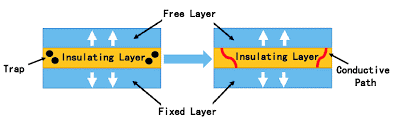
\includegraphics[scale=0.6]{./fig31} % e.g. insert ./image for image.png in the working directory, adjust scale as necessary
\caption{Traps contributing to electron tunnelling in TDDB}
\label{3.31} % insert suitable label, this is used to refer to a fig from within the text as shown above
\end{figure}


\noindent Sometimes, an electron can gain enough energy to overcome the Si-SiO2 interface potential barrier. Once this barrier is breached, electrons are accelerated through the dielectric breaking bonds thus creating traps. The traps increase the tunnelling current through the dielectric by providing a low barrier path across the dielectric to the electrons giving rise to a tunnelling current. This is a positive feedback process. The trap creation increases until the tunnelling current burns a hole in the dielectric.
\subsection{Hot Carrier Damage}
in a MOSFET, after pinch-off the lateral electrical field is restricted to the region between pinch-off and the drain contact. Thus, the electrical field increases as the length decreases increasing the drift current of the electron. This gives rise to hot electrons that may cause impact ionization, HCI, substrate leakage current and trap generation. 
\subsection{Electromigration}
EM refers to the diffusion of metal ions along the direction of electron flow in a conductor. As electrons collide with an aluminium atom, the momentum transfer increases the probability of the atom moving parallel to the electron. As the aluminium atom vacates its initial position, it creates a vacancy and instead diffuses across the conductor to fill a vacancy due to a crystal defect. When the vacancies at the initial position of the aluminium atom are not replenished, it creates a defect there. The defects coalesce to produce a large void that eventually depletes the region of all aluminium atoms in the wire leading to circuit failure.

\section{Short Channel Effects}
Short-Channel Effects refer to the effects that arise in a MOSFET when the channel length is comparable to the size of the source and drain depletion region.
 
\begin{figure}[htb]
\centering
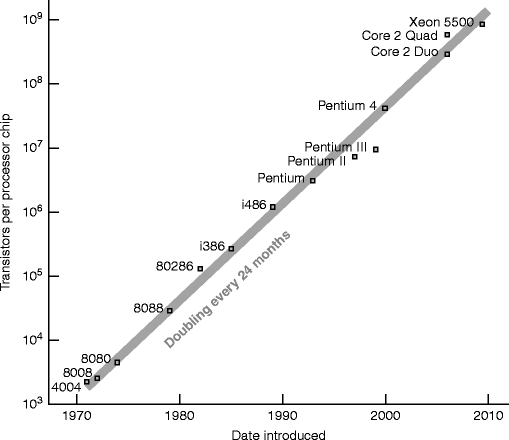
\includegraphics[scale=0.6]{./fig32} % e.g. insert ./image for image.png in the working directory, adjust scale as necessary
\caption{Graph depicting Moore’s law. Transistors per chip v. date
Short-channel effects are inevitable as a consequence of Moore’s law}
\label{3.32} % insert suitable label, this is used to refer to a fig from within the text as shown above
\end{figure}

\subsection{Drain Induced Barrier Lowering}
DIBL refers to the lowering of threshold voltage due to high drain voltage. A high drain voltage reduces the barrier voltage at the source by increasing the forward bias effect allowing easy injection of electrons from the source into the channel. Thus, the drain voltage is inducing a lowering in barrier at the source. A higher drain voltage also reduces the charges the gate voltage must balance by assuming a greater share of it. 
\subsection{Velocity Saturation}
in short channel devices, electric field is usually very high as voltage isn’t scaled linearly with channel length. Drift velocity of an electron increases linearly with electric field. Beyond a certain value of electric field, the drift velocity saturates. An electron in a short-channel device is under high electric field stress. Thus, electrons attain their saturation drift velocity much before the drain saturation voltage. At saturation velocity, the drain current also saturates and therefore current saturation occurs. But current saturation occurs before drain saturation voltage indicating that current saturation occurs as a result of drift velocity saturation and not pinch-off. This reduces the reliability of the device as it no longer saturates at a known value of drain voltage.
\subsection{Quantum Confinement}
At very small device sizes, the device size and de-broglie wavelength of electron become comparable. This implies that laws of classical mechanics no longer apply to the electron and we must use quantum mechanics to determine their behaviour.
\subsection{Hot Carrier Injection}
a hot carrier is a highly energetic charge carrier. Hot carriers are generated by incidence of photons on the substrate that creates a hole and a highly energetic electron called a hot electron. In hot carrier injection, an electron is injected from the n-channel to the gate oxide dielectric increasing its threshold voltage by oxide charging resulting in poor gate control. Holes travel out of the channel via the substrate giving rise to leakage current that can be measured to determine the extent of HCI. Hot electrons also strike the Si-H bonds at the interface generating traps that contribute to further dielectric degradation. HCI is more pronounced at low temperatures as collision probability is greatly reduced at higher temperatures due to increased vibration.
\subsection{Impact Ionization}
hot electrons can collide with other Si atoms generating electron-hole pair and increasing the drain current past saturation. 
\subsection{Mobility Degradation}
as we scale down, vertical electric field increases causing electron scattering at the Si-SiO2 interface reducing mobility of carriers.
\section{NBTI Mechanism}
NBTI is an effect that shifts the threshold voltage for a pMOS when a negative gate bias voltage is applied at elevated temperatures. NBTI arises due to trapped charges at the interface and the oxide layer. The resulting threshold voltage rise leads to a decrease in drain saturation current. The threshold voltage shift increases with stress time and reduces as the stress is removed. This is because threshold voltage shift occurs due to interface and bulk trap charges, as the negative electric field is removed, the charges diffuse back to their initial positions restoring the broken bonds and reducing the threshold voltage shift.
NBTI is more pronounced in (110) crystal lattices that have higher hole mobility due to greater density of Si-H bonds. Addition of Nitrogen induces additional hole traps in the bulk oxide. Thinner oxide layer too contributes to a greater electric field that ultimately leads to a more pronounced NBTI effect. Deuterium and Fluorine help reduce NBTI by replace the Si-H bond with a much stronger bond resulting in lesser trap generation. NBTI can be modelled by the reaction-diffusion and two-stage model. RD model describes the breaking of Si-H interface bonds by holes as a two-way process. Channel holes break the bonds that releases hydrogen that can diffuse through the oxide layer generating a hole trap. The diffusing hydrogen can also get trapped in process-induced bulk traps in the oxide layer. Electron and hole assisted tunnelling can further activate pre-existing traps. Activation of these traps ultimately rises the threshold voltage, degrading the oxide and disrupting operation.

